% !TEX TS-program = XeLaTeX
% use the following command:
% all document files must be coded in UTF-8
\documentclass[english]{textolivre}
% build HTML with: make4ht -e build.lua -c textolivre.cfg -x -u article "fn-in,svg,pic-align"

\journalname{Texto Livre}
\thevolume{15}
%\thenumber{1} % old template
\theyear{2022}
\receiveddate{\DTMdisplaydate{2021}{11}{3}{-1}} % YYYY MM DD
\accepteddate{\DTMdisplaydate{2022}{1}{17}{-1}}
\publisheddate{\DTMdisplaydate{2022}{5}{10}{-1}}
\corrauthor{Anna Beatriz Dimas Furtado}
\articledoi{10.35699/1983-3652.2022.36965}
%\articleid{NNNN} % if the article ID is not the last 5 numbers of its DOI, provide it using \articleid{} commmand 
% list of available sesscions in the journal: articles, dossier, reports, essays, reviews, interviews, editorial
\articlesessionname{articles}
\runningauthor{Furtado and Teixeira} 
%\editorname{Leonardo Araújo} % old template
\sectioneditorname{Daniervelin Pereira}
\layouteditorname{Carolina Garcia}

\title{Multilingual Corpus on Migration and Asylum (COMMIRE): planning, compilation, and overall content}
\othertitle{Corpus Multilíngue sobre Migração e Refúgio (COMMIRE): planejamento, compilação e conteúdo, em linhas gerais}
% if there is a third language title, add here:
%\othertitle{Artikelvorlage zur Einreichung beim Texto Livre Journal}

\author[1]{Anna Beatriz Dimas Furtado \orcid{0000-0002-2801-5146} \thanks{Email: \url{abdimas@gmail.com}}}
\author[2]{Elisa Duarte Teixeira \orcid{0000-0003-3472-3605} \thanks{Email: \url{elisadut@unb.br}}}
\affil[1]{University of Wolverhampton, Faculty of Science and Engineering, School of Mathematics and Computer Science, Wolverhampton, West Midlands, United Kingdom.}
\affil[2]{Universidade de Brasília, Instituto de Letras, Departamento de Línguas Estrangeiras e Tradução, DF, Brasil.}

\addbibresource{article.bib}
% use biber instead of bibtex
% $ biber article

% used to create dummy text for the template file
\definecolor{dark-gray}{gray}{0.35} % color used to display dummy texts
\usepackage{lipsum}
\SetLipsumParListSurrounders{\colorlet{oldcolor}{.}\color{dark-gray}}{\color{oldcolor}}

% used here only to provide the XeLaTeX and BibTeX logos
\usepackage{hologo}

% if you use multirows in a table, include the multirow package
\usepackage{multirow}

% provides sidewaysfigure environment
\usepackage{rotating}

% CUSTOM EPIGRAPH - BEGIN 
%%% https://tex.stackexchange.com/questions/193178/specific-epigraph-style
\usepackage{epigraph}
\renewcommand\textflush{flushright}
\makeatletter
\newlength\epitextskip
\pretocmd{\@epitext}{\em}{}{}
\apptocmd{\@epitext}{\em}{}{}
\patchcmd{\epigraph}{\@epitext{#1}\\}{\@epitext{#1}\\[\epitextskip]}{}{}
\makeatother
\setlength\epigraphrule{0pt}
\setlength\epitextskip{0.5ex}
\setlength\epigraphwidth{.7\textwidth}
% CUSTOM EPIGRAPH - END

% LANGUAGE - BEGIN
% ARABIC
% for languages that use special fonts, you must provide the typeface that will be used
% \setotherlanguage{arabic}
% \newfontfamily\arabicfont[Script=Arabic]{Amiri}
% \newfontfamily\arabicfontsf[Script=Arabic]{Amiri}
% \newfontfamily\arabicfonttt[Script=Arabic]{Amiri}
%
% in the article, to add arabic text use: \textlang{arabic}{ ... }
%
% RUSSIAN
% for russian text we also need to define fonts with support for Cyrillic script
% \usepackage{fontspec}
% \setotherlanguage{russian}
% \newfontfamily\cyrillicfont{Times New Roman}
% \newfontfamily\cyrillicfontsf{Times New Roman}[Script=Cyrillic]
% \newfontfamily\cyrillicfonttt{Times New Roman}[Script=Cyrillic]
%
% in the text use \begin{russian} ... \end{russian}
% LANGUAGE - END

% EMOJIS - BEGIN
% to use emoticons in your manuscript
% https://stackoverflow.com/questions/190145/how-to-insert-emoticons-in-latex/57076064
% using font Symbola, which has full support
% the font may be downloaded at:
% https://dn-works.com/ufas/
% add to preamble:
% \newfontfamily\Symbola{Symbola}
% in the text use:
% {\Symbola }
% EMOJIS - END

% LABEL REFERENCE TO DESCRIPTIVE LIST - BEGIN
% reference itens in a descriptive list using their labels instead of numbers
% insert the code below in the preambule:
%\makeatletter
%\let\orgdescriptionlabel\descriptionlabel
%\renewcommand*{\descriptionlabel}[1]{%
%  \let\orglabel\label
%  \let\label\@gobble
%  \phantomsection
%  \edef\@currentlabel{#1\unskip}%
%  \let\label\orglabel
%  \orgdescriptionlabel{#1}%
%}
%\makeatother
%
% in your document, use as illustraded here:
%\begin{description}
%  \item[first\label{itm1}] this is only an example;
%  % ...  add more items
%\end{description}
% LABEL REFERENCE TO DESCRIPTIVE LIST - END


% add line numbers for submission
%\usepackage{lineno}
%\linenumbers

\usepackage{array}

\begin{document}
\maketitle

\begin{polyabstract}
\begin{abstract}
In recent years, the world has faced an unprecedented migration crisis. "Mobilidades e contatos de línguas" (MOBILANG), a research group at the University of Brasilia focusing on the study of language in the context of migration and asylum, has identified that language is the most significant barrier migrants face in accessing essential services after arriving in Brazil. To mitigate this problem, the group envisioned the creation of a multilingual corpus-driven glossary on the subject aimed at translators, interpreters, those who work with migration, and migrants. The glossary is a partnership with the research group "Terminologia e Tradução Direcionadas por Corpus" (TermiTraDiCo), and has the support of the UNESCO Chair on Language Policies for Multilingualism. The initial stage consisted of compiling a robust electronic corpus to serve as the base for the glossary. This paper aims to describe the planning, compilation, and overall content of this corpus, named \textbf{C}orpus \textbf{M}ultilíngue sobre \textbf{M}igração e \textbf{R}efúgio (Multilingual Corpus on Migration and Asylum) -- COMMIRE, a medium-large corpus containing comparable (and some parallel) texts in Brazilian Portuguese, Spanish, French, and English.

\keywords{Corpus compilation \sep Specialized corpora \sep Corpus-driven terminology \sep Multilingual corpora \sep Migration and asylum}
\end{abstract}

\begin{portuguese}
\begin{abstract}
Nos últimos anos, o mundo tem enfrentado uma crise migratória sem precedentes. O grupo de pesquisa "Mobilidades e contatos de línguas" (MOBILANG), da Universidade de Brasília, dedicado ao estudo da língua em contextos de migração e refúgio, identificou que a barreira linguística é a maior dificuldade que os migrantes enfrentam para acessar serviços básicos no Brasil. Para mitigar esse problema, o grupo planejou a criação de um glossário multilíngue direcionado por corpus sobre o tema, voltado para tradutores, intérpretes, pessoas que trabalham na área e migrantes. O projeto é fruto de uma parceria com o grupo "Terminologia e Tradução Direcionadas por Corpus" (TermiTraDiCo), além de receber o apoio da Cátedra UNESCO em Políticas Linguísticas para o Multilinguismo. A primeira etapa consistiu na compilação de um corpus eletrônico robusto para servir de base para o glossário. Este artigo tem o objetivo de descrever o planejamento, a compilação e as principais características desse corpus, batizado \textbf{C}orpus \textbf{M}ultilíngue sobre \textbf{M}igração e \textbf{R}efúgio -- COMMIRE, um corpus médio-grande contendo textos comparáveis (e alguns paralelos) em português brasileiro, espanhol, francês e inglês.

\keywords{Compilação de corpora \sep Corpus especializado \sep Terminologia direcionada por corpus \sep Corpus multilíngue \sep Migração e refúgio}
\end{abstract}
\end{portuguese}

% if there is another abstract, insert it here using the same scheme
\end{polyabstract}

\section{Introduction}\label{sec-intro}

International migration flows are an ever-growing concern in the present world. The humanitarian situation is currently undergoing one of its most critical moments, considered by the United Nations (UN) as the greatest humanitarian and migratory crisis since 1945. The International Organization for Migration (IOM) estimates that there are approximately 272 million migrants in the world nowadays\footnote{INTERNATIONAL ORGANIZATION FOR MIGRATION. World Migration Report. 2021. Available in: \url{https://publications.iom.int/system/files/pdf/wmr_2020.pdf.} Access on: 02, Nov. 2021.}. According to the 2020 Global Trends report\footnote{UNHCR. Global Trends: Forced Displacement in 2020. June 2021. Available in: \url{https://www.unhcr.org/60b638e37/unhcr-global-trends-2020.} Access on: 02, Nov. 2021.} of the UN Agency for Refugees (UNHCR), adverse conditions have forced 82.4 million people to leave their homes; among them, 26.4 million are now considered refugees, and 4.1 million are asylum seekers\footnote{There is a difference between asylum seekers and refugee migrants. An asylum seeker is someone whose request for asylum is still being processed. Refugees are migrants who were granted the refugee status, meaning that they were entitled to international protection by the country of asylum.}.

Brazil has had a period of substantial growth in its recent history, becoming a popular destination for refugees worldwide, especially from Latin America (Venezuela, Haiti, Cuba) and Africa (Angola, Nigeria, Senegal). In early 2021, CONARE (Brazilian National Committee for Refugees) and the Observatory for International Migration (OBMIGRA) showed in their annual report that the Brazilian government received 28.899 asylum claims in 2020. This is a particularly alarming number for the restrictive context we are currently living in, considering the COVID-19 pandemic and related mobility restrictions \cite[p.~9]{silva_refugio_2021}.

In this context, the MOBILANG\footnote{More information is available at the group’s webpage: \url{http://www.mobilang.unb.br.} Access on: 02, Nov. 2021.}  research group was created at the University of Brasilia to investigate language contact in situations involving human mobility. One of the extension programs of this group, “Migration and Frontiers in the Federal District”, focuses on implementing solutions to promote linguistic and cultural accessibility, and social insertion for the population of migrants and refugees arriving in Brazil. Preliminary investigation of the group has identified poor communication as one of the most common barriers preventing migrants from accessing essential services, as some of them do not speak Portuguese fluently when they arrive in the country \cite{garcia_o_2019,silva_refugio_2021}, and most Brazilians do not speak their languages\footnote{More information about languages spoken in Brazil available in: \url{https://www.ethnologue.com/country/BR/languages.} Access on: 28, Jan. 2021.}.

Among the solutions envisioned to facilitate migrants’ communication in Brazil, especially with governmental and charitable organizations with which they need to interact during the process of asylum-seeking, we proposed the compilation of a multilingual terminological database to support the creation of a freely available glossary on the subject of migration and asylum. The work presented in this paper is connected to this project, developed in partnership with the research group TermiTraDiCo\footnote{More information about the group is available in:  \url{http://www.termitradico.unb.br.}  Access on: 02, Nov. 2021.} (Corpus-Driven Terminology and Translation). Our ultimate goal is to register and disseminate recurrent terminological and linguistic patterns occurring in informative and normative texts, documents, and other materials used in communicative situations involved the sheltering and welcoming of migrants into the  Brazilian culture and society.

An initial and necessary step to create such terminological database is the compilation of an electronic corpus containing linguistic materials that represent, as closely as possible, the texts that most often circulate among people involved and working with migrants, such as government agencies, charitable institutions, community translators, as well as the refugees themselves. In this paper, we describe the process of building the Multilingual Corpus on Migration and Asylum – COMMIRE (\textbf{C}orpus \textbf{M}ultilíngue sobre \textbf{M}igração e \textbf{R}efúgio) and its resulting overall content and linguistic features.

Considering the needs of the MOBILANG group and the theoretical and methodological approaches provided by TermiTraDiCo, we compiled the initial version of the COMMIRE corpus using texts in Brazilian Portuguese, English, French, and Spanish collected in previous projects \cite{furtado_compilacao_2019-1,furtado_compilacao_2019}. Sketch Engine$^®$ \cite{kilgarriff_sketch_2004,kilgarriff_sketch_2021} was used to analyze the corpus content in the four languages.

In the following sections, we will first discuss multilingual corpora regarding the subject area of migration. Then, we will cover the theoretical approach of Corpus Linguistics adopted in this project. Next, we will describe the methodology used for selecting, collecting, preparing, and organizing the texts of COMMIRE. Finally, we will present and discuss the overall content and the main linguistic features of the resulting corpus, commenting on the successful and mistaken decisions, and pointing out the steps currently undertaken to revise and re-balance the initial version of the corpus, which has already been used to compile a beta version of the envisioned Glossary on Migration and Asylum~\cite{furtado_glossario_2019}\footnote{The Glossary can be accessed on TermiTraDiCo's website, under the "Resources" tab (\url{https://tinyurl.com/yckka642}).}.

\section{Multilingual Corpora and Migration}\label{sec-normas}

Technological advancements of the last four decades or so fostered substantial changes in how we communicate. The end of the twentieth century inaugurated the rise of the Information Society, a network-functioning society powered by information \cite{castells_galaxia_2003}. This large amount of electronically available textual information can be systematically collected to build corpora, which now play a crucial role in the development of several tools and services, such as Natural Language Processing (NLP) applications \cite{jurafsky_speech_2009}, including Machine Translation (MT) systems \cite{poibeau_machine_2017}, Speech Recognition (SR) applications \cite{mitkov_speech_2014}, Question-Answering (QA) systems \cite{mitkov_question_2014}, Automated Writing Assistance \cite{mitkov_automated_2014}, and many more.

Regarding the use of corpora in translation, parallel texts are often preferred. There are, however, multiple impediments to the employment of such resource - for example: in less commonly spoken languages, and in overly specialized and/or interdisciplinary domains in which / where the availability of reliable, up-to-date, and extensive parallel corpora is not a reality. A practical solution to overcome this scarcity has been the use of comparable, multilingual resources.

Multilingual corpora can be extensively used in different tasks, but are especially useful in interpreting and translation \cite{mitkov_translation_2015}. They can also be explored to produce databases, termbases, ontologies, glossaries, and dictionaries for translators (id, ibid). This fruitful and close relation between electronic corpora, translation and terminology has been progressing for years \cite{bowker_working_2002}, making the daily work of translators and interpreters much easier.

Despite the increasing availability of resources for specialized translation, some areas have not been covered satisfactorily. This is precisely the case of humanitarian areas, where funding is usually scarce \cite{rico_perez_hacker_2013}, and marketable potential is low. Since this is a somewhat neglected area, there is a widespread common misbelief that by simply digitalizing analogic or printed resources the problem would be solved.

\textcite{rico_perez_tecnologias_2010, rico_perez_hacker_2013} has pointed out an absence of native-electronic resources on migration built specifically for translators, and the situation has not improved much in the last decade. Admittedly, there are corpora available on migration, such as the COMPAS corpus\footnote{More information can be obtained in \url{https://www.sketchengine.eu/compas-corpus/.} Accessed on 02, Nov. 2021.}, in English, or the ISPIE corpus\footnote{More information available in \url{https://preseea.linguas.net/Inicio.aspx.} Accessed on 02, Nov. 2021.}, in Spanish. Nonetheless, these corpora either cover mostly news \textbf{about} migration, or are a \textbf{small} subset to a larger, general-language corpus. Therefore, there is a strong need for a larger, representative corpus on migration and asylum.

Moreover, the migration subject field is vast and interdisciplinary. Genres and text types circulating in social contexts related to the area may differ in terms of register (formal/informal), and linguistic variation (regional and national variants of a language), for example, being subject to the structure of the differing legal systems of the country in which they occur. For example, “\textit{asilo}” in Spanish accounts for “asylum” in English, but in Brazilian Portuguese, the term can mean both “\textit{refúgio}” (an international fundamental right, granted by the 1951 Geneva Convention) and “\textit{asilo político}” (national protection granted to foreigners persecuted for political reasons; it is characteristic of Latin America, and it may not be internationally recognized).

In fact, community interpreters, humanitarian translators, cultural mediators and professionals working in migration are dealing with these people’s fundamental rights. This means that terminological consistency is key to communicating, and can be a matter of life and death. Thus, collecting register- and country-related variation information can be extremely valuable to these users, so they can establish effective communication between the diverse parties involved.

Apart from serving as the source of linguistic information to build terminological databases, a corpus on this area may also prove highly beneficial as a source of information and authentic usage contexts for translators, interpreters, and linguists, as well as researchers, cultural mediators, public workers, training officers, and staff who work with migrants. It can be also helpful to migrants themselves, when filling in the paperwork to claim asylum or reading about their rights and resources, for example.

\section{Corpus Linguistics to Build Multilingual Corpora}\label{sec-modelo}

Corpus Linguistics (CL) is an empirical approach to language that considers it as a probabilistic system \cites{johns_micro-concord:_1986, aijmer_english_1991,svartvik_language_1992}[p.~30]{sardinha_linguistica_2004}; that is, “even though many constructions are possible, some have a greater probability of occurring”\footnote{“Embora muitas construções sejam possíveis, algumas delas têm probabilidade maior de ocorrer”. Translated by the authors.} \cite[p.~20]{tagnin_corpora_2015}. In order to observe this probability of occurrence, an investigation conducted within the CL framework requires large quantities of carefully selected electronic texts called corpora (plural for corpus).  

According to \textcite{bowker_working_2002}, a corpus is a collection of authentic texts in electronic format collected according to specific research criteria. In a previous undergraduate research project \cite{furtado_compilacao_2019}, we systematized some general criteria used by \textcite{bowker_working_2002,teixeira_linguistica_2008} to compile terminological corpora:

\begin{enumerate}[label=\alph*)]
\item Use of authentic texts (they should not be produced to generate linguistic data for research); 
\item Use of natural-occurring texts (usually produced by native speakers); 
\item Texts should represent the area to which they belong (and because of that, usually, the more texts, the better); 
\item Texts should be in electronic format (they must be searchable by computers), and they should meet well-defined criteria for selection (chosen according to a clear research objective);
\end{enumerate}

\textcite[p.~20]{sardinha_linguistica_2004} lists several additional criteria to be taken into account when compiling a corpus, such as:

\begin{enumerate}[label=\alph*)]
\item \textbf{content} – which textual typologies will be collected in which languages, and which linguistic variations should be included?
\item \textbf{internal arrangement} – how will collected materials be organized? A multilingual corpus, for example, can be comparable (when subcorpora share main features such as subject, textual typology, language, and more) or parallel (source texts and their corresponding translation(s) are aligned at the sentence level, to allow the observation of equivalent sentences side by side).
\item \textbf{size} – how many words should be collected so that the corpus is as representative as possible of the language subset being analyzed?
\item \textbf{mode} – will the corpus contain written texts, spoken (speech transcription), or both?
\item \textbf{time} – which time period will it represent?
\item \textbf{authorship} – what kind of authorship will be considered (texts written by native speakers or learners, specialists, or laypeople)?
\item \textbf{purpose} – what texts are relevant for the corpus constitution and/or the research goals?
\item \textbf{language} – are texts in one language (\textbf{monolingual}), two languages (\textbf{bilingual}), or several languages (\textbf{multilingual})?
\item \textbf{encoding} – what kind of extra-linguistic data (bibliographic or data collection information) will be added to the texts in the corpus; will texts be tagged with linguistic information (such as morphological, syntactic, semantic, pragmatic categories)?
\end{enumerate}

One of the main and most crucial features to be observed in corpus compilation is \textbf{representativeness}. As faithfully as possible, the corpus must represent the language produced by the linguistic group and the communicative reality being observed to allow for generalizations \cites[p.~22]{sardinha_linguistica_2004}[p.~164]{teixeira_linguistica_2008}{mcenery_corpus_2012}.

As for attesting whether a corpus is representative of a language or one of its subsets, there is no method so far to determine \textbf{in advance} how many samples of language should be collected to achieve representativeness. Nevertheless, it is possible to adopt a corpus-driven approach to verify whether the corpus is large enough \textbf{after} the collection phase: the ReCor program \cite{seghiri_too_2014}. The software generates graphs containing two lines, a red line (representing alphabetically ordered files), and a blue line (representing randomly ordered files) (id., ibid.). Calculations are based on the Zipf Law and the type/token ratio, indicating that a corpus reaches representativeness when new tokens are not being included, from a statistic standpoint, in amounts significant enough to alter the curves (ibid.). Therefore, a corpus can be considered to be representative when the curves approximate to 0.5 in the type/token (Ty/To) axis (ibid.).

Another essential aspect to be considered is \textbf{corpus balancing}, especially in the case of comparable corpora. A balanced comparable corpus usually has a similar number of tokens, similar text typologies, genres, and linguistic varieties across languages \cite{sardinha_linguistica_2004,teixeira_linguistica_2008} to allow comparisons. It might be the case that the size and typology of texts vary among languages and/or among cultures within the same language. However, the departing point in building a comparable corpus is to look for similar textual features across languages when collecting texts to build the corpus.

It is generally accepted that the study of language using electronic corpora can be corpus-based or corpus-driven. The first uses electronic corpora as a major source of data to investigate previously established theories or linguistic hypotheses, i.e., CL is used more as a methodology \cites[p.~1084]{tagnin_producao_2009}[p.~5-6]{mcenery_corpus_2012}. On the other hand, corpus-driven studies explore corpus data using tools specially designed for corpus research (introduced ahead), and the linguistic data they provide are the primary source of observation and theorization about linguistic phenomena. In that sense, CL is more of an approach, a particular way of viewing language – as a probabilistic system – and how it works, which is revealed through the data provided by the corpus \cites[p.~1084]{tagnin_producao_2009}[p.~6]{mcenery_corpus_2012}.

This research adopts a corpus-driven approach. This means, for example, that we decided to rely on usage to choose texts for the corpus, instead of consulting area experts to determine a domain tree upon which the corpus would be structured – a methodology generally used in corpus-based Terminology.

Furthermore, since our main goal was to collect texts representing the language used in the area being studied as proposed by \textcite{tagnin_translator-oriented_2012}, we chose texts being used every day by the community of migrants, refugees, and people working with this audience. This way, our corpus would have a greater chance of being a representative sample of the most recurrent features of the language used by these populations.

\section{CL tools to explore the corpus}\label{sec-organizacao}

Computational tools available for the observation and exploration of electronic corpora, apart from the special features that set them apart, share some basic functionalities commonly used in CL studies -- described in-depth in: \textcite{fromm_wordsmith_2020,rodriguez_martinez_extraccion_2021}, such as:

\begin{description}
\item[Wordlists:] list the words contained in one or more texts of the corpus in decreasing or increasing order of occurrences, in alphabetical order from the beginning, or from the end of the word, among other options, depending on the software being used. They also allow the generation of lists of word clusters (also known as n-grams) with two or more items.

\item[Keyword lists:] generate a list of key words in a corpus, obtained by comparing the wordlist of a corpus of study with the wordlist of a larger corpus (at least five times larger, usually), called reference corpus. These lists are often ordered by “keyness” – a measure indicating the probability of the relatively higher frequency of an item in the study corpus be the result of chance or not – illustrated in the “Score” columns in \Cref{Table01} where "F" stands for Frequency". The keyword list helps with the initial identification of the main topic of the text(s) and/or corpus.


% \begin{figure}[htbp]
% \centering
% 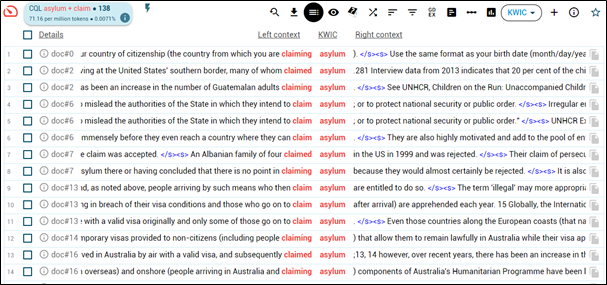
\includegraphics[width=\textwidth]{Figura01.png}
% \caption{First ten keywords\protect\footnotemark of the COMMIRE corpus.}
% \label{Figura01}
% \source {authors’ elaboration.}
% \footnotetext{Reference corpora used in this paper are selected by default in Sketch Engine; They belong to the TenTen corpus family. More information available in: \url{https://www.sketchengine.eu/documentation/tenten-corpora/.} Accessed on 02 Jan. 2022.}
% \end{figure}

\begin{sidewaystable}
%\begin{table}[htbp]
%\caption{First ten keywords\protect\footnotemark of the COMMIRE corpus.}
\caption{First ten keywords of the COMMIRE corpus.}
\label{Table01}
\begin{tabular}{@{}lllllllllllll@{}}
\toprule
& \multicolumn{3}{c}{\textbf{Portuguese}} & \multicolumn{3}{c}{\textbf{English}} & \multicolumn{3}{c}{\textbf{French}} &
\multicolumn{3}{c}{\textbf{Spanish}} \\
& \textbf{Keyword} & \textbf{Score} & \textbf{F} & \textbf{Keyword} & \textbf{Score} & \textbf{F} & \textbf{Keyword} & \textbf{Score} &
\textbf{F} & \textbf{Keyword} & \textbf{Score} & \textbf{F} \\
1 & ACNUR & 1,222.523 & 2,833 & asylum-seeker & 999.626 & 2.771 & OSAR &
643.238 & 861 & reasentamienlo & 909.815 & 1,852\\
2 & CONARE & 1,008.69 & 1,378 & UNHCR & 887.895 & 4,405 & asile &
496.416 & 7,251 & ACNUR & 772.617 & 2,793\\
3 & apátrida & 911.821 & 1,531 & asylum & 671.349 & 13.236 & CGRA &
426.305 & 577 & reasentar & 620.092 & 958\\
4 & refugiado & 839.847 & 6,487 & RSD & 523.886 & 1.330 & OFPRA & 404.41
& 690 & refugiados & 523.99 & 1,582\\
5 & refugiados & 806.208 & 1,799 & resettlement & 303.853 & 1.589 &
UNHCR & 279.82 & 591 & asilo & 451.818 & 4,447\\
6 & apatridia & 660.657 & 834 & refugee & 288.384 & 16.354 & réfugié-e-s
& 252.56 & 336 & refugiado & 424.84 & 9,009\\
7 & solicitante & 523.755 & 1,942 & seeker & 277.985 & 4.773 & réfugier
& 184.597 & 6,341 & solicitante & 179.111 & 2,689\\
8 & reassentamento & 410.633 & 862 & stateless & 210.328 & 725 &
subsidiaire & 156.069 & 439 & apátrida & 110.318 & 226\\
9 & refúgio & 357.093 & 3,129 & unaccompanied & 173.984 & 709 & apatride
& 129.707 & 297 & refugiar & 95.301 & 1,073\\
10 & refugiar & 240.433 & 1,804 & statelessness & 122.927 & 273 & traite
& 122.329 & 1,757 & asilado & 68.64 & 108\\
\bottomrule
\end{tabular}
\source {authors’ elaboration.}
\notes{Reference corpora used in this paper are selected by default in Sketch Engine; they belong to the TenTen corpus family.\\More information available in: \url{https://www.sketchengine.eu/documentation/tenten-corpora/.} Accessed on 02 Jan. 2022.}
%\end{table}
\end{sidewaystable}
%\footnotetext{Reference corpora used in this paper are selected by default in Sketch Engine; they belong to the TenTen corpus family. More information available in: \url{https://www.sketchengine.eu/documentation/tenten-corpora/.} Accessed on 02 Jan. 2022.}


\item[Concordance lists:] show context lines in which the query word/expression appears, centralized and/or highlighted (\Cref{Figura01}), accompanied by its immediate context on the left and on the right. They can be generated in monolingual or multilingual corpora. Some concordance tools also allow the reordering of context lines by the words occurring on the neighborhood of the search word / expression, left or right, and/or the listing of the words that co-occur most often on the left or on the right contexts (called “collocates”), making the identification of recurrent patterns easier. Some tools allow the exploration of aligned parallel corpora, showing the context of a search word/expression side-by-side with (or on top of) its equivalent context lines in the target language(s) corpus.

\begin{figure}[htbp]
\centering
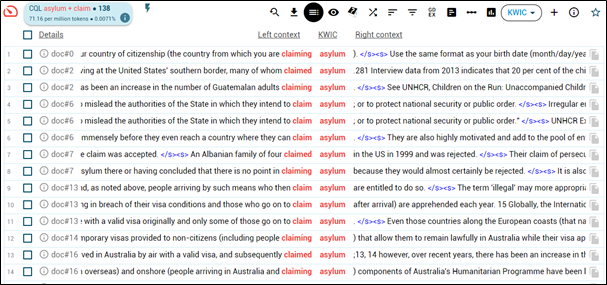
\includegraphics[width=\textwidth]{Figura01.png}
\caption{Example of a concordance list result screen in Sketch Engine®.}
\label{Figura01}
\source {authors’ elaboration.}
\end{figure}

\item[Regular expression search:] enables the search for complex linguistic patterns by using special symbols\footnote{More information available in: \url{https://www.sketchengine.eu/guide/regular-expressions/.} Accessed on 02 Jan. 2022.}. It is possible to look for words finishing in *ing, for example, or phrases fitting in the pattern ADJ + NP. In Sketch Engine, regular expressions can be used in concordance searches to fit in word-level patterns, or as a part of the Corpus Query Language (CQL) to investigate complex patterns. In \Cref{Figura02}, we are searching for phrases fitting in the ADJ + asylum + NN pattern. The CQL query can be seen in the blue box at top, on the left side of the screen.

\begin{figure}[htbp]
\centering
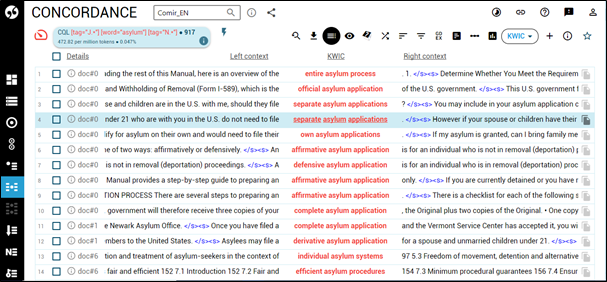
\includegraphics[width=\textwidth]{Figura02.png}
\caption{Example of an CQL query in the Concordance lines.}
\label{Figura02}
\source {authors’ elaboration.}
\end{figure}


\end{description}

For our initial exploration of the corpus, we chose to work with \textit{Sketch Engine} \cite{kilgarriff_sketch_2004}, as described in section 6. In the following section, we present the methodology we adopted to select, collect, and compile the texts comprising this first version of COMMIRE.

\section{The Compilation of COMMIRE}

Before starting collecting texts for a corpus, it is essential to plan its intended content. This plan will guide the process of selecting and capturing its texts, as emphasized by \textcite{bowker_working_2002,teixeira_linguistica_2008}. Based on the criteria previously described, we planned our corpus to reflect the features summarized in \Cref{Table02}.

\begin{table}[htbp]
\caption{Criteria used in the planning of the COMMIRE corpus.}
\begin{tabular}{lp{10cm}}
\toprule
Criterion & Features  \\
\midrule
Language & Multilingual (in Portuguese, Spanish, French, and English). \\
Textual typologies & Focus on booklets, guides, and questionnaires available to asylum seekers and refugees, first. Then, if needed, manuals and scientific journals aimed at people working with refugees may be included. \\
Corpus type & Comparable (most texts originally written in each language) and partially parallel (translations are welcome when collected from reliable sources detailing the material’s provenience.) \\
Size & Medium-large (at least 1-million words in each language, 4 million words total.) \\
Mode & Written texts aimed at refugees, asylum seekers, migrants and people working with this audience. \\
Sources & Government, International Organizations (IOs), Non-governmental Organizations (NGOs), and other institutions assisting or working with this audience.\\
Knowledge domain & Migration and asylum-seeking.\\
Authorship & Written or published by the institutions defined in Source.\\
Publishing Date & Recent (published in or after 2005.). \\
Encoding & Files converted into plain text format (.txt) encoded in UTF-8; add a header containing bibliographic and collection data; automatic morphosyntactic annotation to be carried out by the software chosen to explore the corpus, Sketch Engine \cite{kilgarriff_sketch_2004}. \\ 
\bottomrule
\end{tabular}
\label{Table02}
\source{authors’ elaboration.}
\end{table}

After the planning phase, the compilation takes place. It consists of searching for the material, then downloading the files, preprocessing, and finally storing them, as systematized in \textcite{seghiri_metodologiprotocolizada_2011,sanchez_ramos_corpus_2019,sanchez_ramos_documentacion_2020}. Keeping the set criteria in mind, we searched and manually selected electronic texts focusing on: i) informing and/or describing how the process of asylum-seeking occurs in the countries of destination where the chosen languages are spoken; ii) instructions on how to claim asylum; and iii) documents required to do so. Initially, we used the following queries to search for these materials on the Internet, in the four languages of the project:

\begin{itemize}
\item \textit{“como solicitar refúgio,” “material para solicitação de refúgio”}
\item \textit{“comment demander asile,” “conseils sur la demande d'asile"}
\item \textit{“how to claim asylum,” “guidance on claiming asylum”.}
\item \textit{“solicitud de refugio,” “orientación sobre la solicitud de asilo”.}
\end{itemize}

We collected the materials, in .pdf format, provided by Google search engine, which ranks its pages using their own unique criteria, in the order they appeared in the results. Google’s search mechanism favors, among other criteria\footnote{GOOGLE. How Search Works. Available in: \url{https://www.google.com/search/howsearchworks/.} Access on 02, Nov. 2021.}, the exhibition of pages that users access more frequently, which was something quintessential for this research, as our goal was to collect texts used on a daily basis by the target audience (migrants, refugees, their translators, interpreters, and other people working in institutions involved in the welcoming of migrants).

All the files collected are freely available on the Internet and were produced institutionally and collectively by the government of the respective countries, international organizations (such as UNHCR) or NGOs responsible for sheltering refugees, asylum seekers or migrants. It is important to highlight that journal articles (of informative nature, produced by experts in the area) were written by different authors, despite the fact that some were downloaded from unique sources.

Once all the files were collected for the four languages, the next step consisted of converting them into plain text files (.txt), UTF-8 encoded. Some files were “dead pdfs” (image only) and had to go through optical character recognition (OCR), performed with the premium version of \textit{Abbyy Fine Reader}\footnote{ Available in: \url{https://www.abbyy.com/pt-br/finereader/.} Access on 02, Nov. 2021.}  (Abbyy from now on). Once in .txt, we pasted a header on each file and filled it out with bibliographical and retrieval information.

Some of the files, collected for a preliminary study \cite{furtado_primeiros_2017,furtado_compilacao_2019}, were also added to this corpus. They consisted of texts written in Brazilian Portuguese and their respective translations into the other three working languages, namely, two informative booklets distributed by the Brazilian Migratory Police (\textit{Polícia Federal}), and four questionnaires electronically available for asylum-seekers. The material was also translated into Arabic, but due to the use of non-Latin alphabet and our lack of knowledge on this language, we did not use it in the project. We opted for aligning the source texts with the respective translations at the sentence level, as explained in \textcite{furtado_compilacao_2019}.

\section{Using Sketch Engine to Explore COMMIRE}

In order to explore the corpus, we uploaded it into Sketch Engine® \cite{kilgarriff_sketch_2004}, a software built to manage and analyze electronic corpora developed by Lexical Computing Ltd. and available since 2003 – SKE from now on. Once uploaded, the corpus can be accessed on any computer connected to the Internet. We chose this software because it handles multilingual corpora well, in addition to having several large corpora integrated into it. Some were used as reference for the comparisons when we were generating keywords and term-candidates lists. SKE was also chosen because it has, besides the essential tools cited in section 2, some features that are unique and especially useful for glossary building and for identifying recurring language patterns – such as Word Sketches. This tool summarizes the lexical and grammatical behavior of a word or query based on a tagged and lemmatized\footnote{To lemmatize a corpus is to gather all wordforms under their lemma form. “A lemma is a group of wordforms that are related by being inflectional forms of the same base word. The lemma is usually labeled by that base or stem. So, for instance, in English destroy, destroys, destroying and destroyed are all part of the verb lemma destroy.” \cite[p.~245]{mcenery_corpus_2012}.}  version of the corpus, as shown in \Cref{Figura03}.

\begin{figure}[htbp]
\centering
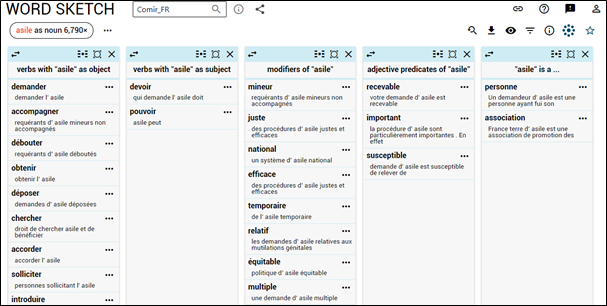
\includegraphics[width=\textwidth]{Figura03.png}
\caption{Word Sketches for the french word “\textit{asile}”.}
\label{Figura03}
\source{authors’ elaboration.}
\end{figure}

SKE offers a one-month trial including the upload of corpora of up to one million words. As COMMIRE is larger than that, we acquired a premium license for academic use to conclude the research herein described.

Next, we present the main features of the compiled corpus, followed by a brief discussion of its applicability and adequacy to our initial objective: serve as the base to create a multilingual, corpus-driven glossary on asylum and migration.

\section{Results: Overview of COMMIRE Data}

We noticed during the text collection step that materials aimed at refugees and asylum seekers are far less common than materials aimed at the people who work with them. One possible reason for that is the sensitive nature of the work, which demands comprehensive training and qualification of the staff and collaborators involved. Futhermore, it may implicate that the balancing of the corpus may be compromised by the availability of materials on the Internet, our only source of texts so far.

An important fact to be highlighted is that manually selecting and collecting texts can be quite demanding and time-consuming, as the material must be thoroughly analyzed in terms of source and publishing details, such as authorship, translation and editing authorship, nationality of writer/translator (when possible), publication dates, etc. Nevertheless, checking this information before including any of the texts in the corpus increases the reliability of the resulting data. On the other hand, even though our initial planning indicated that texts should all be converted from .pdf to .txt files, only a small part was actually converted, due to constraints imposed by time and by the complexity involved in the collection process. Fortunately, another advantage of SKE is allowing the processing of texts in .pdf format, even though it may generate some noise in the results, such as the inclusion of broken words and symbols in the wordlists.

SKE applies its own OCR to the .pdf files, but similarly to Abbyy, the disposition of graphic elements and text formatting (these files usually contain several visual resources) does not always work, and many automatically converted .txt files needed manual edition to correct broken words, clean unnecessary symbols, and set pagination, for example. This treatment was only applied to the files that we had time to transform into .txt (see below), at the time. \Cref{Table03} presents the number of types and tokens obtained in each language, according to Sketch Engine® parameters (including treated and non-treated texts).

\begin{table}[htbp]
\centering
\caption{Total types and tokens of COMMIRE by language.}
\begin{tabular}{ lccccc } 
\toprule
Language & Types & Tokens & T/T Ratio \\
\midrule
Brazilian Portuguese & 57,071 & 1,494,954 & 0.038 \\ 
Spanish & 50,026 & 1,323,436 & 0.038 \\
French & 43,472 & 1,326,563 & 0.033 \\
English & 59,667 & 2,109,352 & 0.028 \\
%\midrule
\textbf{Total} & \textbf{210,236} & \textbf{6,254,305} & \\
\bottomrule
\end{tabular}
\label{Table03}
\source{authors’ elaboration.}
\end{table}

As previously mentioned, COMMIRE includes some parallel texts aligned at the sentence level, resulting from a preliminary study \cite{furtado_primeiros_2017,furtado_compilacao_2019-1,furtado_glossario_2019}. However, these texts represent only 1.5\% of the whole corpus. \Cref{Table04} presents COMMIRE data divided into two subcorpora: comparable (containing only texts originally written in one of the corpus languages) and parallel (texts written originally in Brazilian Portuguese and their corresponding translations into the other three working languages).

\begin{table}[htbp]
\centering
\caption{COMMIRE types and tokens by subcorpus and language.}
\begin{tabular}{lcccc}
\toprule
 & \multicolumn{2}{c}{Comparable subcorpus} & \multicolumn{2}{c}{Parallel subcorpus} \\
Language & Types & Tokens & Types & Tokens \\
\midrule
Brazilian Portuguese & 54,583 & 1,477,349 & 2,488 & 17,605 \\
Spanish & 47,437 & 1,305,011 & 2,589 & 18,425 \\
French & 40,866 & 1,306,553 & 2,606 & 20,010 \\
English & 57,332 & 2,091,482 & 2,335 & 17,870 \\
%\midrule
\textbf{Total} &\textbf{200,218} & \textbf{6,180,395} & \textbf{10,018} & \textbf{73,910} \\
\bottomrule
\end{tabular}
\label{Table04}
\source{authors’ elaboration.}
\end{table}

It is important to point out the possible imprecision in the number of types and tokens provided by the software, as most files were inserted into SKE in .pdf. The software uses metadata from files to calculate the number of types in the corpus and then calculates the number of tokens based on the number of white spaces\footnote{Learn more about it in \url{https://www.sketchengine.eu/my_keywords/token/.} Access on 02, Nov. 2021.}. However, in the process of optical recognition, several symbols are generated, such as the insertion of extra white spaces and characters, resulting from formatting marks, or hyphenated words that became two different words. This elevates the number of wrongfully added white spaces, which interferes with the calculation of types and tokens, shown in \Cref{Figura04}. The number of tokens in the files that have already been converted into UTF-8 coded plain text (.txt), though, is precise.

\begin{figure}[htbp]
\centering
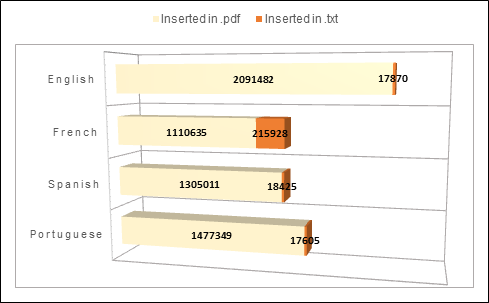
\includegraphics[width=0.85\textwidth]{Figura04.png}
\caption{Number tokens in .pdf and .txt in COMMIRE's first version.}
\label{Figura04}
\source{authors’ elaboration.}
\end{figure}

\Cref{Figura04} shows that approximately 4.5\% of COMMIRE texts (the equivalent to 270,95 tokens) were, in fact, converted into .txt and manually edited to correct OCR conversion problems. French has the largest number of treated texts because it was the language we first applied manual treatment of files. All the files in the parallel subcorpus are already in UTF-8 coded, plain text format.

During the collection, we observed that some text types (briefly describe below) are more recurrent than others:

\begin{enumerate}[label=\alph*)]
\item \textbf{Reports and technical documents} – texts generally aimed at eligibility officials and/or people working with migrants.

\item \textbf{Academic publications} – papers in scientific journals focusing on disseminating specialized know\-ledge to scholars, NGOs and officials of governmental institutions working with migrants.

\item \textbf{Manuals} – instructional files explaining the routine of how to deal with asylum claims, aimed at officials and people working with migrants.

\item \textbf{Teaching materials} – books and materials for language teaching directed to the migrant audience.

\item \textbf{Forms} – distributed to those who are going to claim asylum and/or initiate the asylum-seeking process.

\item \textbf{Booklets and guides} – informative material, often lavishly illustrated and written in accessible language, aiming at migrants wishing to initiate their asylum-seeking process.
\end{enumerate}

At first, we considered booklets and guides as different materials, but a detailed analysis of the content revealed that they are very similar materials, both focusing on informing about something on a clear and simple way, often using several visual resources. Thus, even though the collected texts are configured differently, depending on the text type, they all have an informative purpose, except for the forms. \Cref{Table05} presents the number of tokens and files (in parenthesis) collected in each of the aforementioned text types in the total corpus. \Cref{Figura05} shows the percentage of tokens by text type in each language of the corpus.

\begin{table}[htbp]
\caption{Number of tokens (and files) per text typology and language in COMMIRE}
\begin{tabular}{>{\raggedright}p{3cm}rrrr}
\toprule
Textual typology & \multicolumn{1}{p{2.8cm}}{Brazilian Portuguese} & French & Spanish & English \\
\midrule
Reports and documents & 313,782 (4) & 44,419 (14) & 439,227 (4) & 684,523 (20) \\
Academic publications & 509,121 (14) & 573,851 (31) & 0 &	0 \\
Manuals & 596,554 (9) & 154,652 (8) & 736,543 (16) &	925,177 (27) \\
Language Teaching materials	& 44,964 (6) & 0 &	0 &	0 \\
Forms &	16,114 (9) & 9,258 (5) & 8,614 (4) & 8,169 (4)\\
Booklets and guides & 14,419 (4) & 544,383 (42) &	139,052 (48) & 491,423 (56) \\
\textbf{Total} &	1,494,954 (46) & 1,326,563 (100) &	1,323,436 (72) &	2,109,292 (107) \\
\bottomrule
\end{tabular}
\label{Table05}
\source{authors’ elaboration.}
\end{table}

\begin{figure}[htbp]
\centering
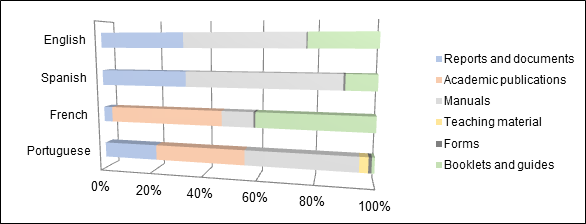
\includegraphics[width=0.85\textwidth]{Figura05.png}
\caption{Percentage of tokens by text type in each language in COMMIRE.}
\label{Figura05}
\source{authors’ elaboration.}
\end{figure}

In order to verify the representativeness of the corpus, we used the ReCor \cite{seghiri_too_2014} software. \Cref{Figura06}, \Cref{Figura07}, \Cref{Figura08} and \Cref{Figura09} describe representativeness for each subcorpus. The curves did not reach the mark of 0.5 in the type/token (Ty/To) axis, indicating that COMMIRE has yet to achieve representativeness, as we expected. Therefore, the corpus needs some adjustments and the addition of new texts to become more balanced and to achieve representativeness. Moreover, \Cref{Figura06} indicates that the Brazilian Portuguese subcorpus is the closest one from achieving representativeness.

The availability of materials in the area of migration and asylum on the Internet is not balanced in all languages, because it depends mostly on governmental policies, especially in the case of materials of high dissemination that need translation, such as booklets and guides for those seeking asylum. Moreover, in many cases, some materials are only made available in printed version. Therefore, there is a disparity in the number of words for collected materials for each text type (for example, booklets, forms, etc.) per language, criterion initially used in an attempt to balance the corpus.

The Brazilian Portuguese corpus, for example, comprises 46 files, six of which are original texts from the parallel subcorpus (two booklets and four forms). \Cref{Table05} shows that there are more files in academic publications and only a few booklets and guides in Portuguese compared to the other languages. One of the reasons for these numbers is that the Portuguese corpus contains texts in Brazilian Portuguese only, whereas the other languages include files from several countries where that language is officially spoken. Furthermore, we observed that Brazil comparatively produced fewer booklets for asylum seekers and refugees but, apparently, invested heavily in producing manuals for employees working with migratory issues.

\begin{figure}[htbp]
\centering
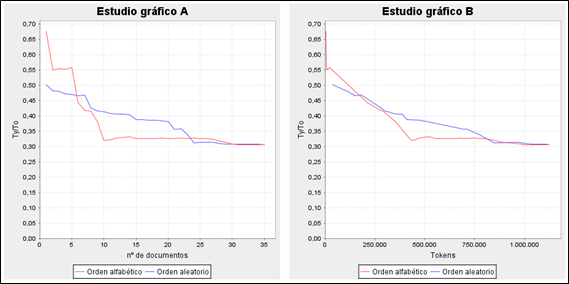
\includegraphics[width=0.85\textwidth]{Figura06.png}
\caption{Representativeness in the Brazilian Portuguese subcorpus.}
\label{Figura06}
\source{authors’ elaboration.}
\end{figure}

It is worth mentioning that manuals and academic publications (such as a book of essays produced by several specialists in the area) are the materials that have the highest number of types. This occurs because they present much information in a more extended format. On the other hand, forms have less linguistic data and are more repetitive, which means its representativeness can be achieved with fewer document samples.

\begin{figure}[htbp]
\centering
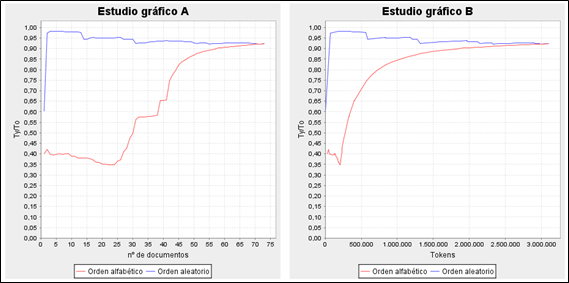
\includegraphics[width=0.85\textwidth]{Figura07.png}
\caption{Representativeness in the French subcorpus. }
\label{Figura07}
\source{authors’ elaboration.}
\end{figure}

The French corpus contains 100 files (six are translations of the parallel corpus originally written in Brazilian Portuguese). Texts come from several francophone countries: Belgium, France, Canada, Luxembourg, Switzerland, plus one file produced in French in Portugal. We also searched for files from francophone Africa, but most of the few we found were not originally written in French, but in Arabic and other less commonly spoken local languages. There are several specialized journal issues in this subcorpus, such as \textit{Planète Éxil}\footnote{Available in: \url{https://www.osar.ch/publications/planete-exil.html.} Access on 02, Nov. 2021.}, published in several volumes – a partnership with international organizations, especially the UN. The journal’s board of editors invites specialists in the area (from several nationalities), as well as refugees and asylum seekers to write about migration and have francophone editors as volunteers.

\begin{figure}[htbp]
\centering
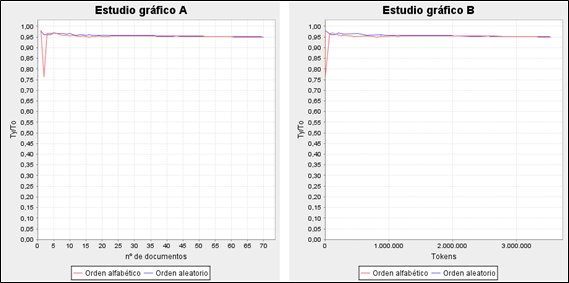
\includegraphics[width=0.85\textwidth]{Figura08.png}
\caption{Representativeness in the Spanish subcorpus.}
\label{Figura08}
\source{authors’ elaboration.}
\end{figure}

The Spanish corpus has 72 files (6 belong to the parallel corpus) from these countries: Mexico, Peru, Spain, Colombia, Ecuador, Costa Rica, Chile, Argentina, Panama, Guatemala, and Uruguay.

It was much easier, as previously mentioned, to find booklets and guides in Spanish, French, and English because we checked several countries, whereas for Brazilian Portuguese, searching was restricted to Brazil only. Nevertheless, we can argue that the main criterion we used for text selection was “opportunistic”, in the sense that availability and easiness of finding them on the Internet were key factors, as we were hoping to simulate the experience of the majority of people looking for information. Producing a glossary that will be effectively used by those who seek these materials on the Internet means providing translators, interpreters and migrants with the terminology occurring in the materials they will consult, use, and/or translate on a daily basis. However, we ended up having to balance the corpus, especially in French, since the booklets we found had fewer words, leading us to add other text types to the French subcorpus so as to reach a number of tokens similar to the other corpora.

\begin{figure}[htbp]
\centering
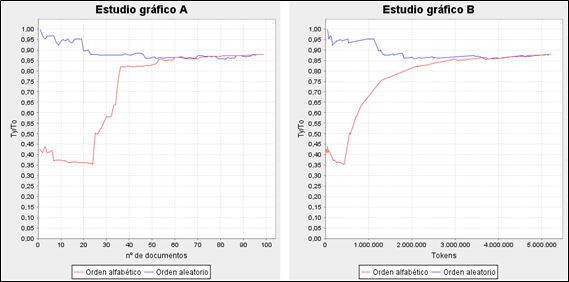
\includegraphics[width=0.85\textwidth]{Figura09.png}
\caption{Representativeness in the English subcorpus.}
\label{Figura09}
\source{authors’ elaboration.}
\end{figure}

Finally, the English subcorpus has 107 files (six in the parallel corpus) from the following countries: United States, Canada, Australia, United Kingdom (England, North Ireland, Great Britain, and Scotland), Ireland, New Zealand, Swiss, South Africa, Trinidad and Tobago, Germany, Philippines, Switzerland, Malta and Egypt.

English is currently seen as a “lingua franca” \cite{hoffman_spread_2000}, and that accounts for the fact that its presence on the Internet is far more abundant than other languages, as there is much more content being produced and publicized in this language. That made it easier for us collect data in this language; as a result, this subcorpus has the largest number of types and tokens. In our search, we noticed a significantly higher occurrence of guides and manuals in English, compared to other text types and to other languages.

\section{Final considerations}

In this paper, we describe the initial steps of a project aiming at the creation of a multilingual glossary on migration and asylum, for which we proposed the compilation of a corpus to serve as the departing point, the COMMIRE – Multilingual Corpus on Migration and Asylum, a multilingual comparable and partially parallel corpus in Brazilian Portuguese, Spanish, French, and English. To build this corpus, we used the theoretical and methodological approach of Corpus Linguistics, based on its probabilistic view of language, which relies on the use of electronically searchable, authentic texts to study language.

In order to conduct the preliminary exploration of the resulting data, we used Sketch Engine \cite{kilgarriff_sketch_2004}, which enabled an optimal usage of the materials, especially because it allows the upload of texts in .pdf format for the analysis. As we have mentioned in the Introduction, COMMIRE was effectively used in a senior undergraduate thesis to compile the prototype of an online corpus-driven Glossary on Migration and Asylum \cite{furtado_glossario_2019}, proving to be very useful to extract specialized language patterns.

Compiling COMMIRE took longer than we anticipated, because of the careful, manual selection of relevant texts. Nonetheless, the resulting corpus is a reliable source of materials available on the Internet on migration and asylum-seeking in the four languages of our research, and will be a good departing point to build the multilingual glossary we are working on.

As limiting factors to the undertaking of this research, we highlight the difficulty of collecting texts in .pdf format and converting them into .txt, a step we could not apply to all the materials gathered due to the prolonged time required for the task. Fortunately, the software we chose for the exploration allows the insertion of .pdf files, making the initial exploration of the corpus possible, even though the type and token counts may not be perfectly reliable.

We are currently working on converting the remaining .pdf texts into .txt, on the cleaning process to eliminate noise derived from conversion and OCR, and on the insertion of headings to all these converted files. As we continue the insertion of new entries to the Glossary, we also identified the need to work on the expansion and re-balance of the corpus – the next step we will be taking. Moreover, as our plan has always been to make an open, up-to-date corpus, so we intend to expand COMMIRE and divide its typologies and varieties in order to investigate representativeness in depth.

One final, vital step will be making the COMMIRE corpus freely available for consultation, which is already in the making. Until then, people interested in using COMMIRE for academic research can contact the authors to request access to the files.

We certainly hope COMMIRE can be systematically expanded by future collaborators, and kept updated and balanced, to continue to be a trustworthy source of information on the areas of migration and asylum-seeking.



\printbibliography\label{sec-bib}


\begin{contributors}[sec-contributors]
\authorcontribution{Anna Beatriz Dimas Furtado}[conceptualization,datacuration,formalanalysis,investigation,methodology,projadm,software,visualization,writing]
\authorcontribution{Elisa Duarte Teixeira}[conceptualization,datacuration,methodology,projadm,supervision,writing]
\end{contributors}



\end{document}

